
\documentclass[progress]{cmpreport}
\usepackage{hyperref}
\newcommand{\head}[1]{\textnormal{\textbf{#1}}} %Used for tables
\usepackage{fontenc}  % \textsterling for £
\usepackage{caption}

\title{Designing, Building, Coding and Tracking a Mechanical Hand/Arm}
\author{Deborah Taylor}
\registration{100085169}

\supervisor{Dr Graeme Richards}
\date{\today}
\ccode{CMP-6013Y}

\summary{Draft as of \today.}
\acknowledgements{}

% If the figures do not fit on one page, comment this line out
\onePageLists
%\linespread{1.5}
\bibliographystyle{apalike} 

% Prevents author/year errors
\usepackage{natbib}
\usepackage{float}
\usepackage{rotating}
\usepackage[strings]{underscore}


\begin {document}


\section{Introduction}
Since the first industrial arm was built in 1954, by George C. Devol\footnote{George Charles Devol, Jr. American Inventor born 20 Feb 1912 and died 11 Aug 2011}, the majority have been claw based and aren't very dexterous or flexible. Due to their design restrictions they can only perform precise, repetitive tasks and are liable to fail if the claws are not aligned correctly, or one stops working. \citep{devol}, \citep{grigorediscovering}.  

To increase manoeuvrability and flexibility, while also reducing restrictions, the mechanical arm needs to be redesigned so it can replicate the majority of movement in a normal human hand, instead of using a claw. 

The purpose of this project is to build a bespoke mechanical (robotic) human skeletal hand/arm, code\footnote{Code and coding are other names for programming. Programming is a way of entering instructions into a machine to execute commands.} it to pick up and put down items using relevant fingers on the hand and track items or movement. This will enable the project to develop a flexible hand that will continue to work, even if one of the fingers is broken or not in alignment. 


\section{Motivation and Aims}
\subsection{Motivation}
 
Prosthetic limbs have been an interest, ever since the author's school friend developed meningitis at an early age and ended up losing an arm. The author saw how difficult it was for that person to complete even the simplest task, such as dressing or tying a shoelace. 

With current skill levels and the project time-frame, it will not be feasible to develop a fully functioning prosthetic limb, therefore, the author has shifted focus to commercial uses instead. Commercial arms are more straight forward to develop and are used in a multitude of industries from manufacturing to defusing bombs. 

This project will, therefore, enable the author to develop their skills (a possible precursor to moving forward into health research and prosthetics) while still producing a project that can be useful commercially.  

\subsection{Aims}
The main aim of the project, as mentioned in the introduction, is to design and build a mechanical hand/arm, with coding that enables it to demonstrate the flexibility and functionality of a human hand. 

The hardware will be able to complete basic tasks such as moving each finger, moving the arm/hand up, down, left and right, plus, picking up and putting down an item. It will, also, have more complex coding to play "Rock, Paper, Scissors" or solve the "Towers of Hanoi puzzle". 

The author is still in the process of identifying which of these two options will be the most suitable for this project, so the design and build has been completed so either can be coded, at a later date. Whichever option is chosen, any missing movement from the other one can be incorporated into the basic coding, to ensure full flexibility is demonstrated. 

\section{Design and Hardware Build}

An online Trello board has been created to log each task, within the project. This enables the author to continually monitor progress and ensure all tasks are completed correctly. To view this Trello board access: https://trello.com/b/cdHgyGX0.

This project involves both hardware and software so a Software Engineering Design Document is needed to show designs, development and testing\footnote{A Design Document is a technical guide for Developers and includes Definitions, Requirements, Use Cases, etc.}. This is the best way to make sure each stage of the design and build is completed correctly and efficiently \citep{mcelrath}.

\subsection{Design}

The full Design Document is too large to include in this report, so an overview is covered here.

\subsubsection{Similar Systems Analysis}
One of the first stages in designing any hardware and software is to investigate and review similar products, to see which features are available and how they differ from the new one being designed. 

This ensures there is no crossover of hardware or software already in existence and helps clarify specifications, requirements and scope, when discussing with a customer. This is also a way to identify if there are any "off the shelf" hardware or software that can be used and, if not, whether there is anything currently in use that be adapted for the new project.

See figure 1 below for analysis of five mechanical arms already in use:

\begin{figure}[H] 
	\caption{Analysis of 5 different mechanical arms}
	\centering
	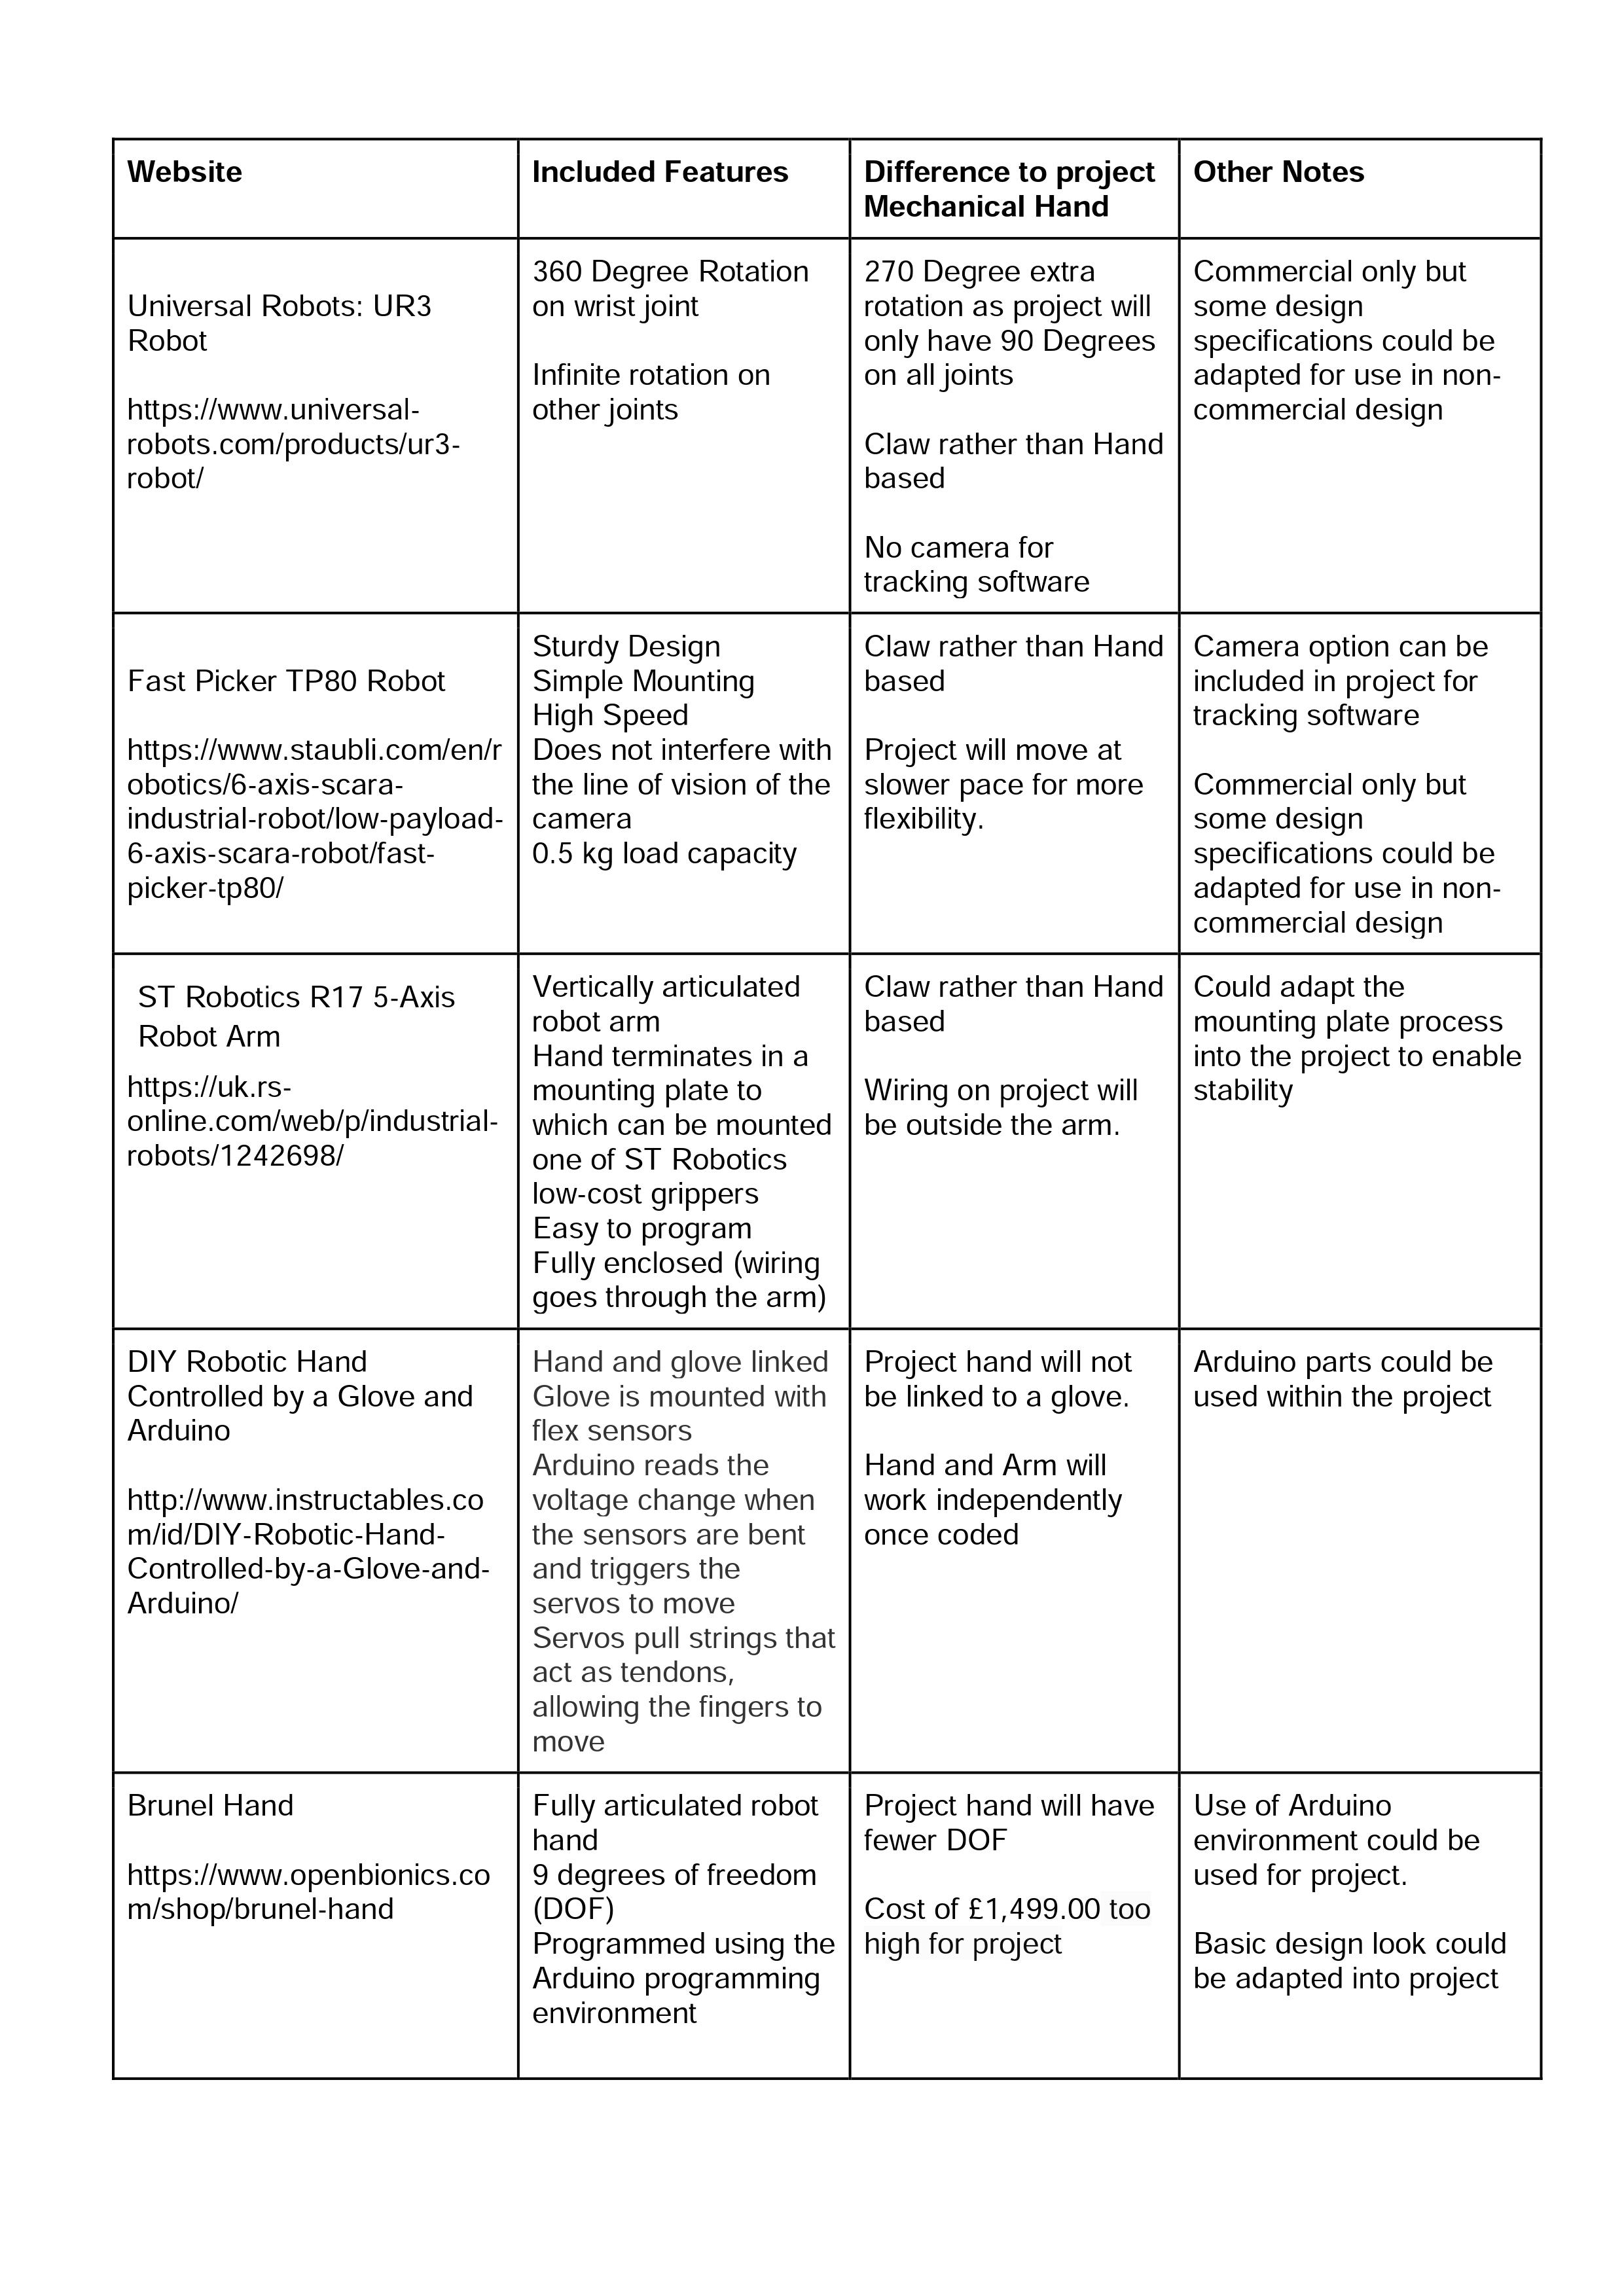
\includegraphics[trim=0cm 2.8cm 0cm 0.15cm, width=1 \textwidth, height=0.75 \textheight]{photos/SSA.jpg}
\end{figure}

\subsubsection{MoSCoW Analysis:}
Once the \textit{Similar Systems Analysis} is completed the next stage is the \textit{MoSCoW Analysis}.

This process determines the different requirements that will be in and out of scope for the project, along with how they should be prioritised for development. 

This analysis is made up of \textit{Must Have, Should Have, Could Have, Won't Have} tasks. \newline

\textbf{\underline{Must Have:}} 

The \textbf{\textit{Must Have}} tasks are identified as absolutely crucial, at base level, for the project to work. These will be prioritised within development and the \textit{Should Have} section will not be started until these are fully completed and tested. 

\begin{itemize}
	\item \textit{Skeletal hand design and arm (up to the equivalent of an elbow)}
	\item \textit{Fingers and thumb that can move independently and/or together}
	\item \textit{Movement rotation of 90 degrees, up, down, left and right}
	\item \textit{Basic coding to enable movement of the arm: up, down, left and right}
	\item \textit{Basic coding to enable the hand to pick up, hold and put down an item}  \newline
\end{itemize} 

\textbf{\underline{Should Have:}} 

The \textbf{\textit{Should Have}} tasks are identified as necessary to the project to increase effectiveness within the design. These are the second stage of a development and will only be started, completed and tested, once the \textit{Must Have} tasks are working correctly.

\begin{itemize}	
	\item \textit{Complex coding to enable hardware to play Rock, Paper, Scissors or solve Towers of Hanoi puzzle}
	\item \textit{Sensor or Camera connected to the hardware (with or without a wire) to identify items or movement} \newline
\end{itemize}	

\textbf{\underline{Could Have:}}
 
The \textbf{\textit{Could Have}} tasks are identified as nice to have, but not necessary for the project to be successful. These are tasks which are desired and may be implemented, depending on cost and the time-frame available. 
\begin{itemize}	
	\item \textit{Ability to move independently of a PC or laptop (utilising a servo controller mounted on the arm)}
	\item \textit{Haptic sensors to enable feedback on how the hand grips an item} \newline
\end{itemize}

\textbf{\underline{Won't Have:}} 

The \textbf{\textit{Won't Have}} tasks are identified to be out of scope for the project and will not be implemented. If the project were to continue into a future development stage, these could be implemented then.  

\begin{itemize}		
	\item \textit{Independent thought and movement eg Artificial Intelligence } 
\end{itemize}

\subsubsection{Use Case (UML) Diagram:}

Once the \textit{MoSCoW} analysis is completed a \textit{Use Case (UML) Diagram}\footnote{Unified Modelling language (UML) is a standard modelling language for developers to visualize and document tasks} is designed to show User interaction with the hardware \citep{AljamaanLBGF14}. From the above \textit{MoSCoW Analysis}, the priorities (to enable the hand to play either Rock, Paper, Scissors or solve the Towers of Hanoi) are identified as:

\begin{itemize}		
	\item \textit{Move arm/hand up, down, left, right and open, close the hand}
	\item \textit{Move fingers independently and/or together so items can be picked up and put down}
	\item \textit{Use a sensor or camera to track items and/or movement}
\end{itemize}

As these priorities are necessary to the project, they need to be added to the \textit{Use Case UML Diagram}, to show how they interact and link together. See figure 2 below: 

\begin{figure}[H] 
	\caption{Use Case UML Diagram }
	\centering
	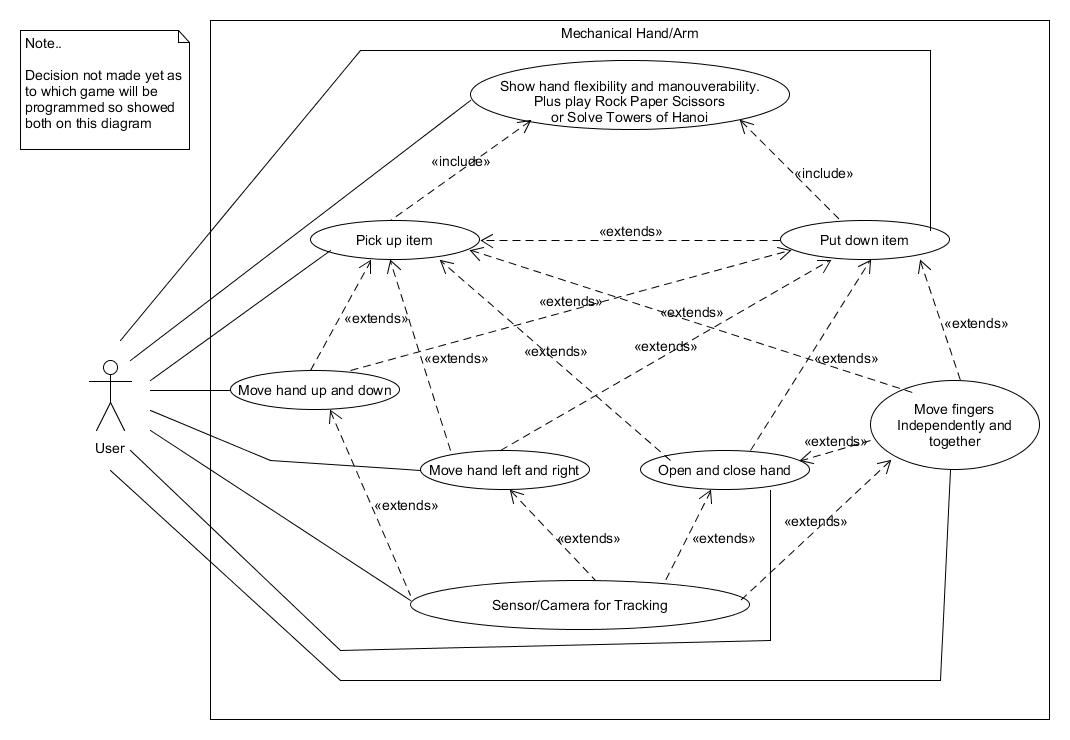
\includegraphics[width=0.8 \textwidth, height=0.535 \textheight]{photos/UMLdiagram.jpg}
\end{figure}

\subsubsection{Use Case Descriptions:}

Following completion of the \textit{Use Case UML Diagram}, \textit{Use Case Descriptions} are written, for each of the tasks shown on the diagram. See below for an example:

\begin{itemize}		
	\item \textit{Use Case 3 Open Hand: describes the process of connecting the laptop signal to the Hand hardware and enabling the Hand to open. This is a basic command that will be fundamental to the Hand movement for later, more complex, coding.}
\end{itemize}

\subsubsection{Detailed Use Case:}

The descriptions are then expanded into \textit{Detailed Use Cases}. These show steps required to achieve each task eg triggers, frequency, release schedules and provide information needed for development. See figure 3 below for an example:

\begin{figure}[H] 
	\caption{Use Case3: Open Hand Example}
	\centering
	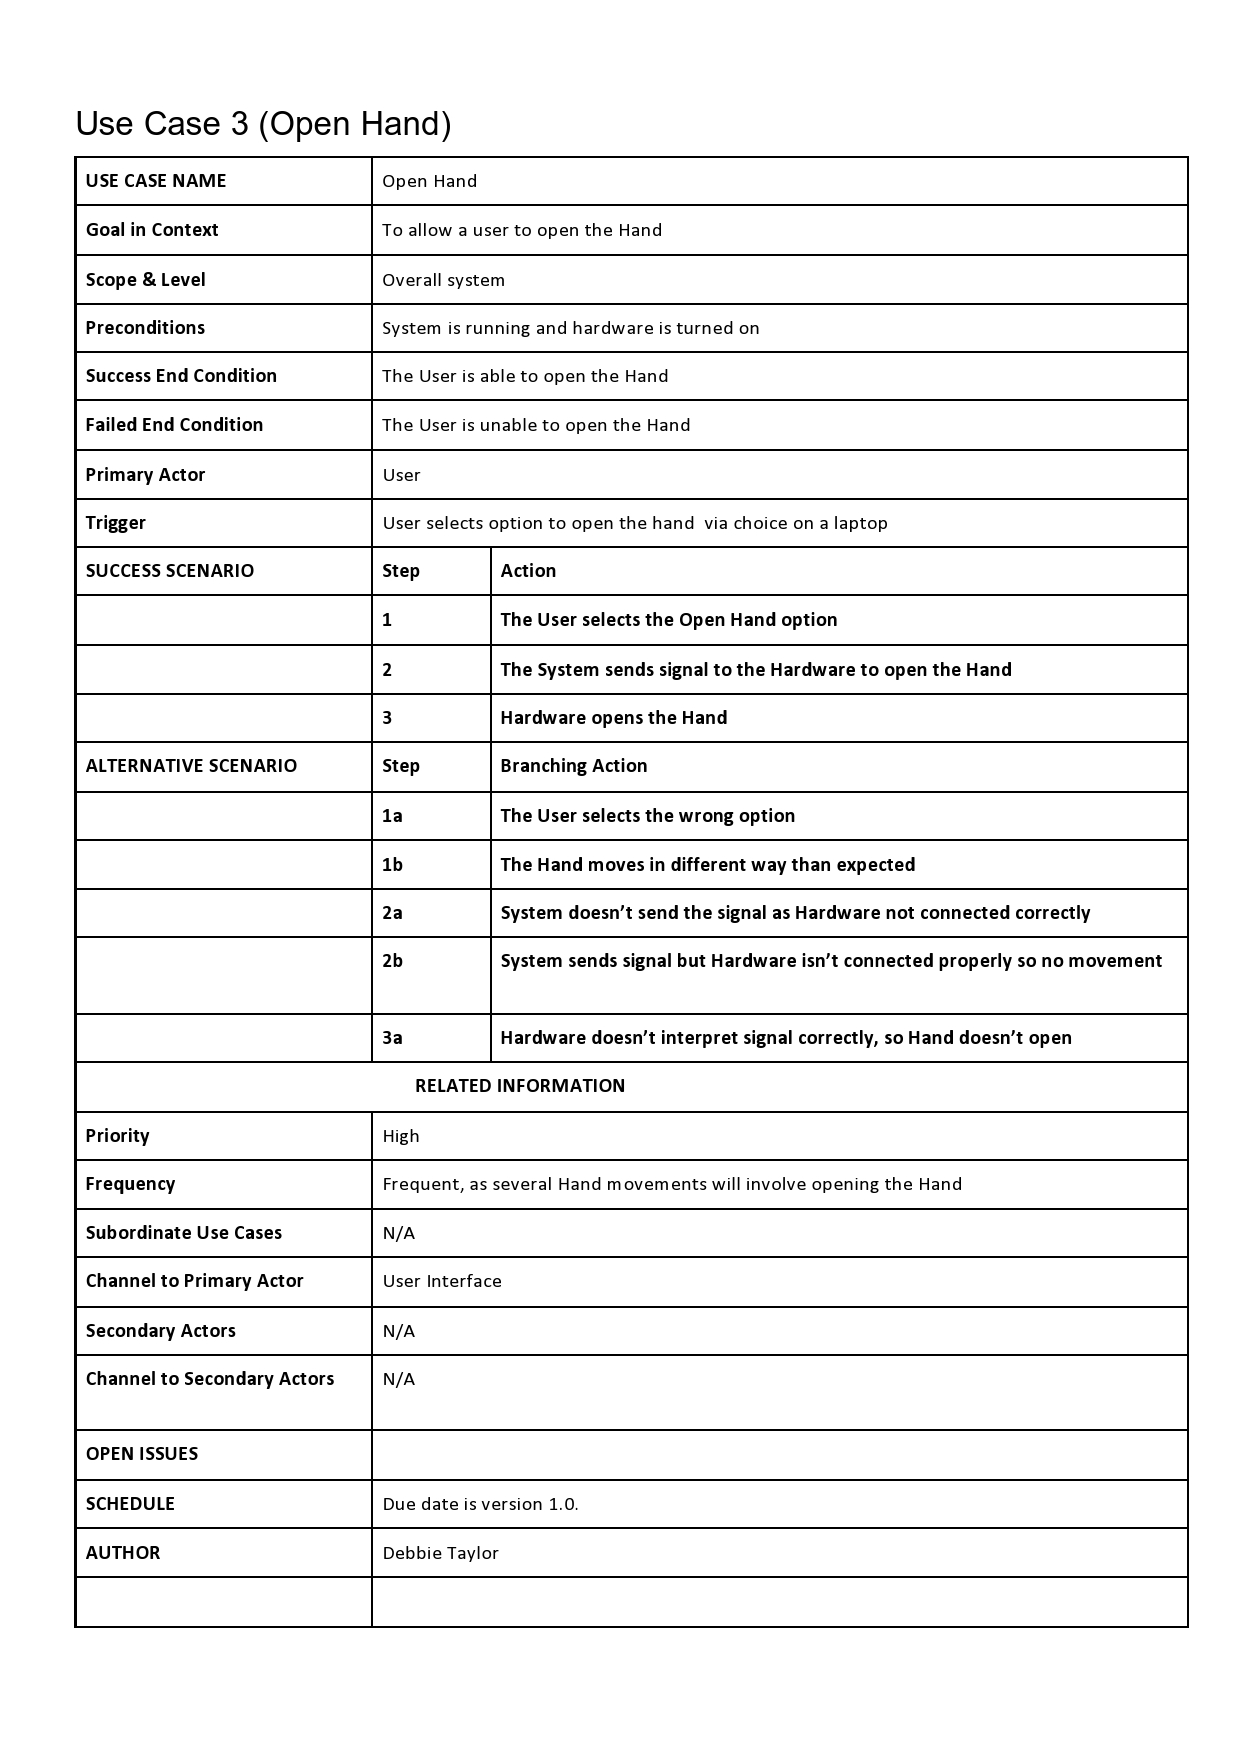
\includegraphics[trim=0cm 7cm 0cm 0.63cm, width=0.9 \textwidth, height=0.629 \textheight]{photos/UseCase_OpenHand.jpg}
\end{figure}

\subsubsection{Sequence Diagram:}

Once the \textit{Detailed Use Cases} are completed the final stage\footnote{As this is a hardware and software design there is no need for Architecture diagrams} is to create \textit{Sequence Diagrams}. These show step by step representations of specific scenarios. See figure 4 below for an example: 

\begin{figure}[H] 
	\caption{Sequence Diagram Example }
	\centering
	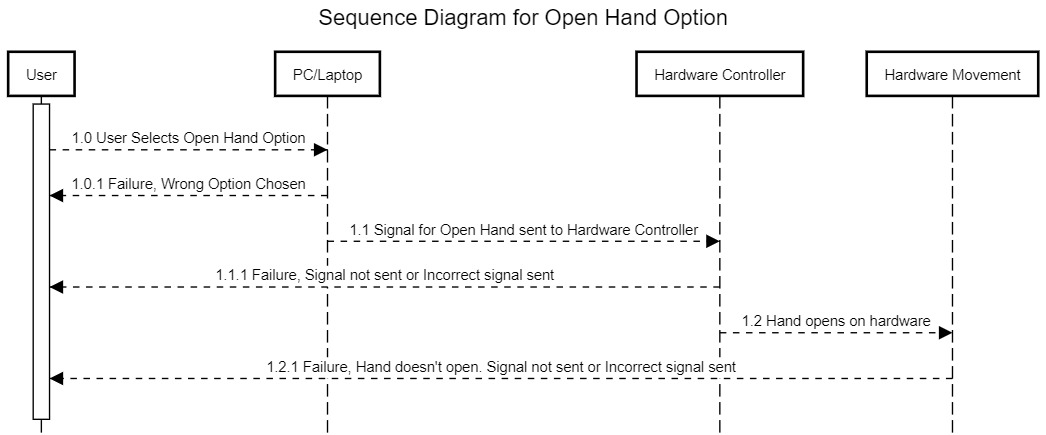
\includegraphics[width=0.9 \textwidth, height=0.45 \textheight]{photos/sequence_diagram.jpg}
\end{figure}

Completing this Design Document confirms there is no "off the shelf" skeletal hand/arm hardware available, so a bespoke build is required for this project.

\subsection{Hardware Build}
The first stage of the build involves identifying how a human hand works. 

In order for a hand to open, close, move each finger, hold items etc, a combination of the fingers and thumb need to be working in sequence \citep{freivalds2011biomechanics}. The author, therefore, needs to investigate the skeletal structure, by reading up on human anatomy and learning the names and connections for each part of a hand 

\subsubsection{Skeletal Human Hand Investigation:}

Identifying this information enables the author to specify exactly which metal shapes need to be cut and how many servos, joints etc are needed to build the hardware.

See figure 5\footnote {Source: http://visual.merriam-webster.com/human-being/anatomy/skeleton/hand.php} below for the picture the author used to identify the shapes needed to build a skeletal human hand:

\begin{figure}[H] 
	\centering
	\caption{Bones and Joints of the Human Hand.} 
	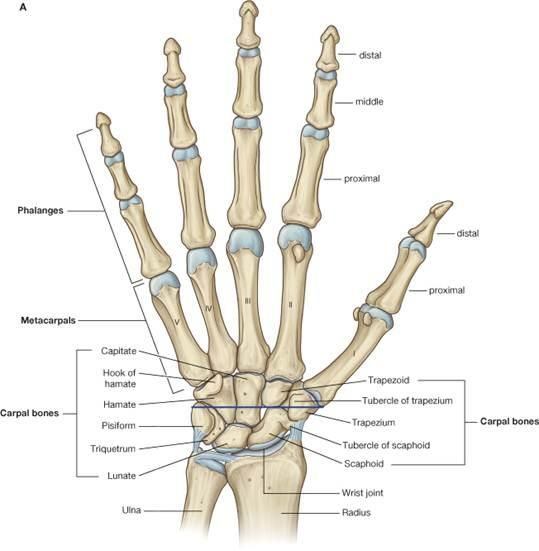
\includegraphics[height=0.45\textheight, keepaspectratio]{photos/hand.jpg} 
\end{figure}

 A friend (who is a machinist) supplies the bespoke metal skeleton "bone" parts, from specifications provided by the author. The rest of the equipment (eg Arduino servos, wiring, sensors and a Polulo servo controller unit for mounting on the arm etc) can be obtained separately "off the shelf", using some of the ideas obtained from the \textit{Similar Systems Analysis}.

\subsubsection{Hardware Build Progress:}

Due to the hardware being fundamental to the project, the build starts during the summer holidays and continues until the middle of Semester 1. Multiple photographs are taken showing step by step progress. See figure 6 and 7 below for a selection of four photographs showing the build as it progresses: 

\begin{figure}[H]
	\centering
	\caption{Hardware Build Progress - Zero to hand built }
	\begin{tabular}{ll}
		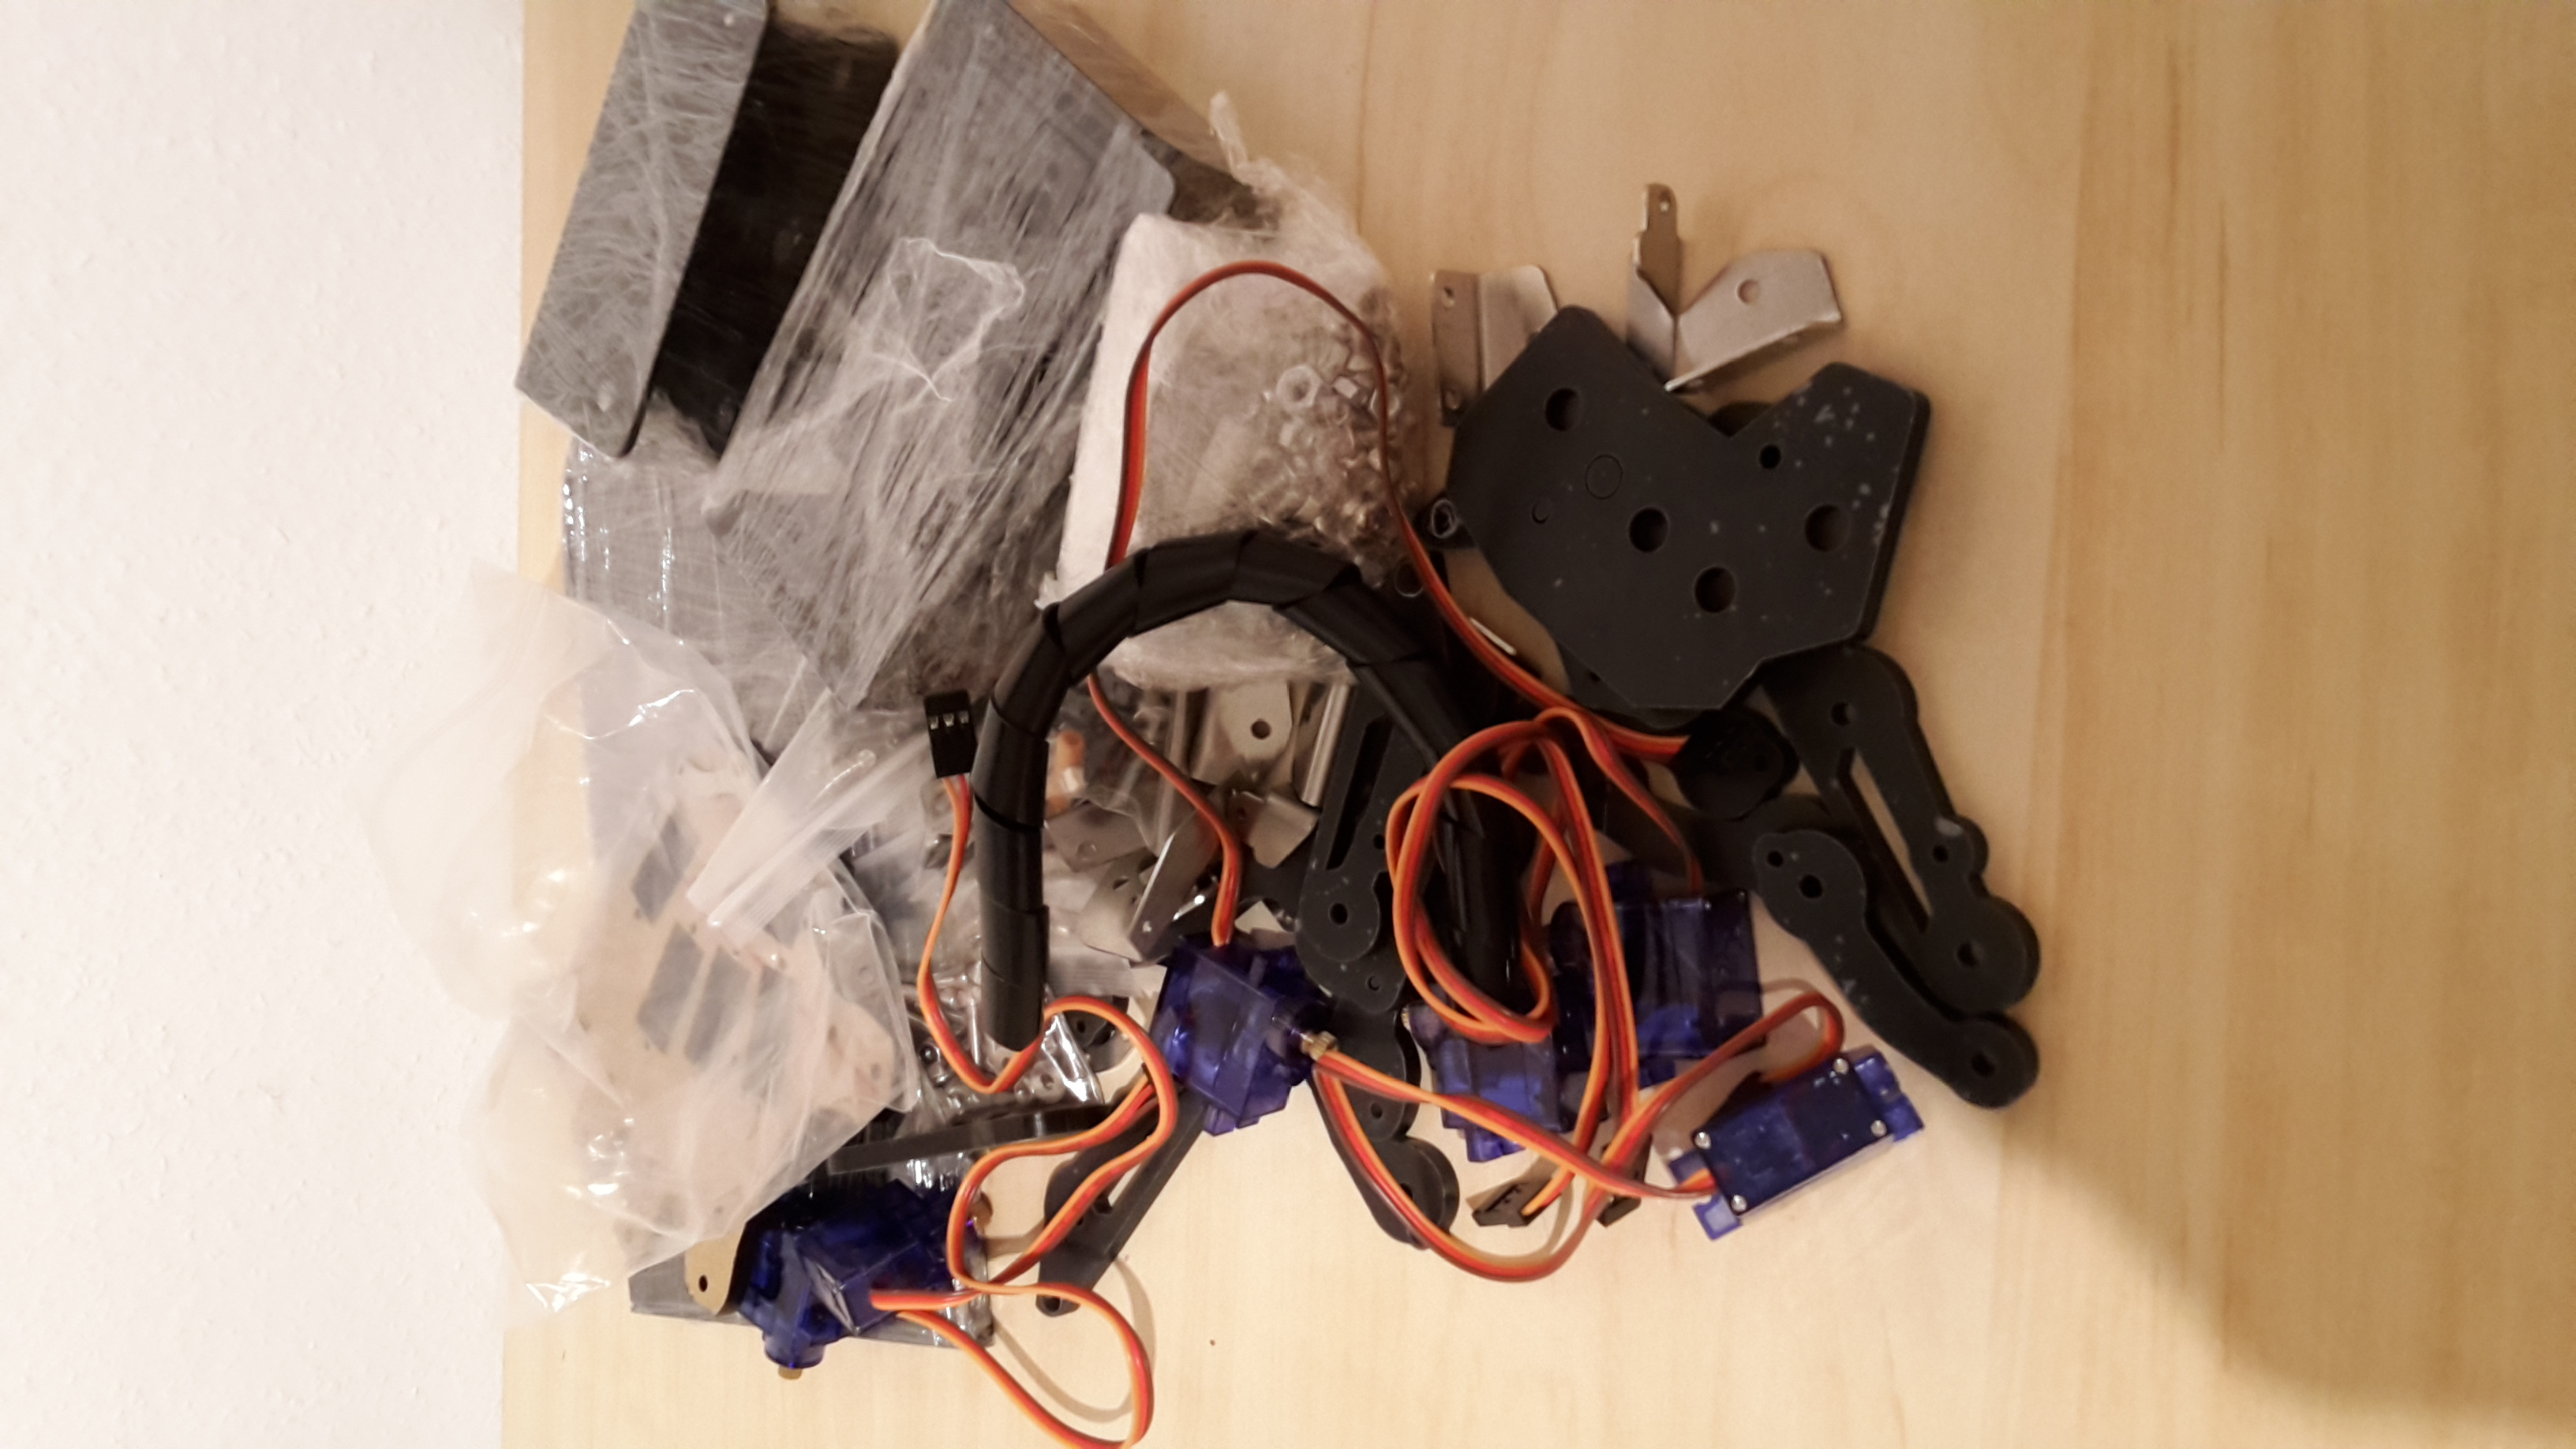
\includegraphics[trim=20cm 0cm 22cm 0cm, clip=true, totalheight=0.28\textheight, angle=-90]{photos/start.jpg}
		&
		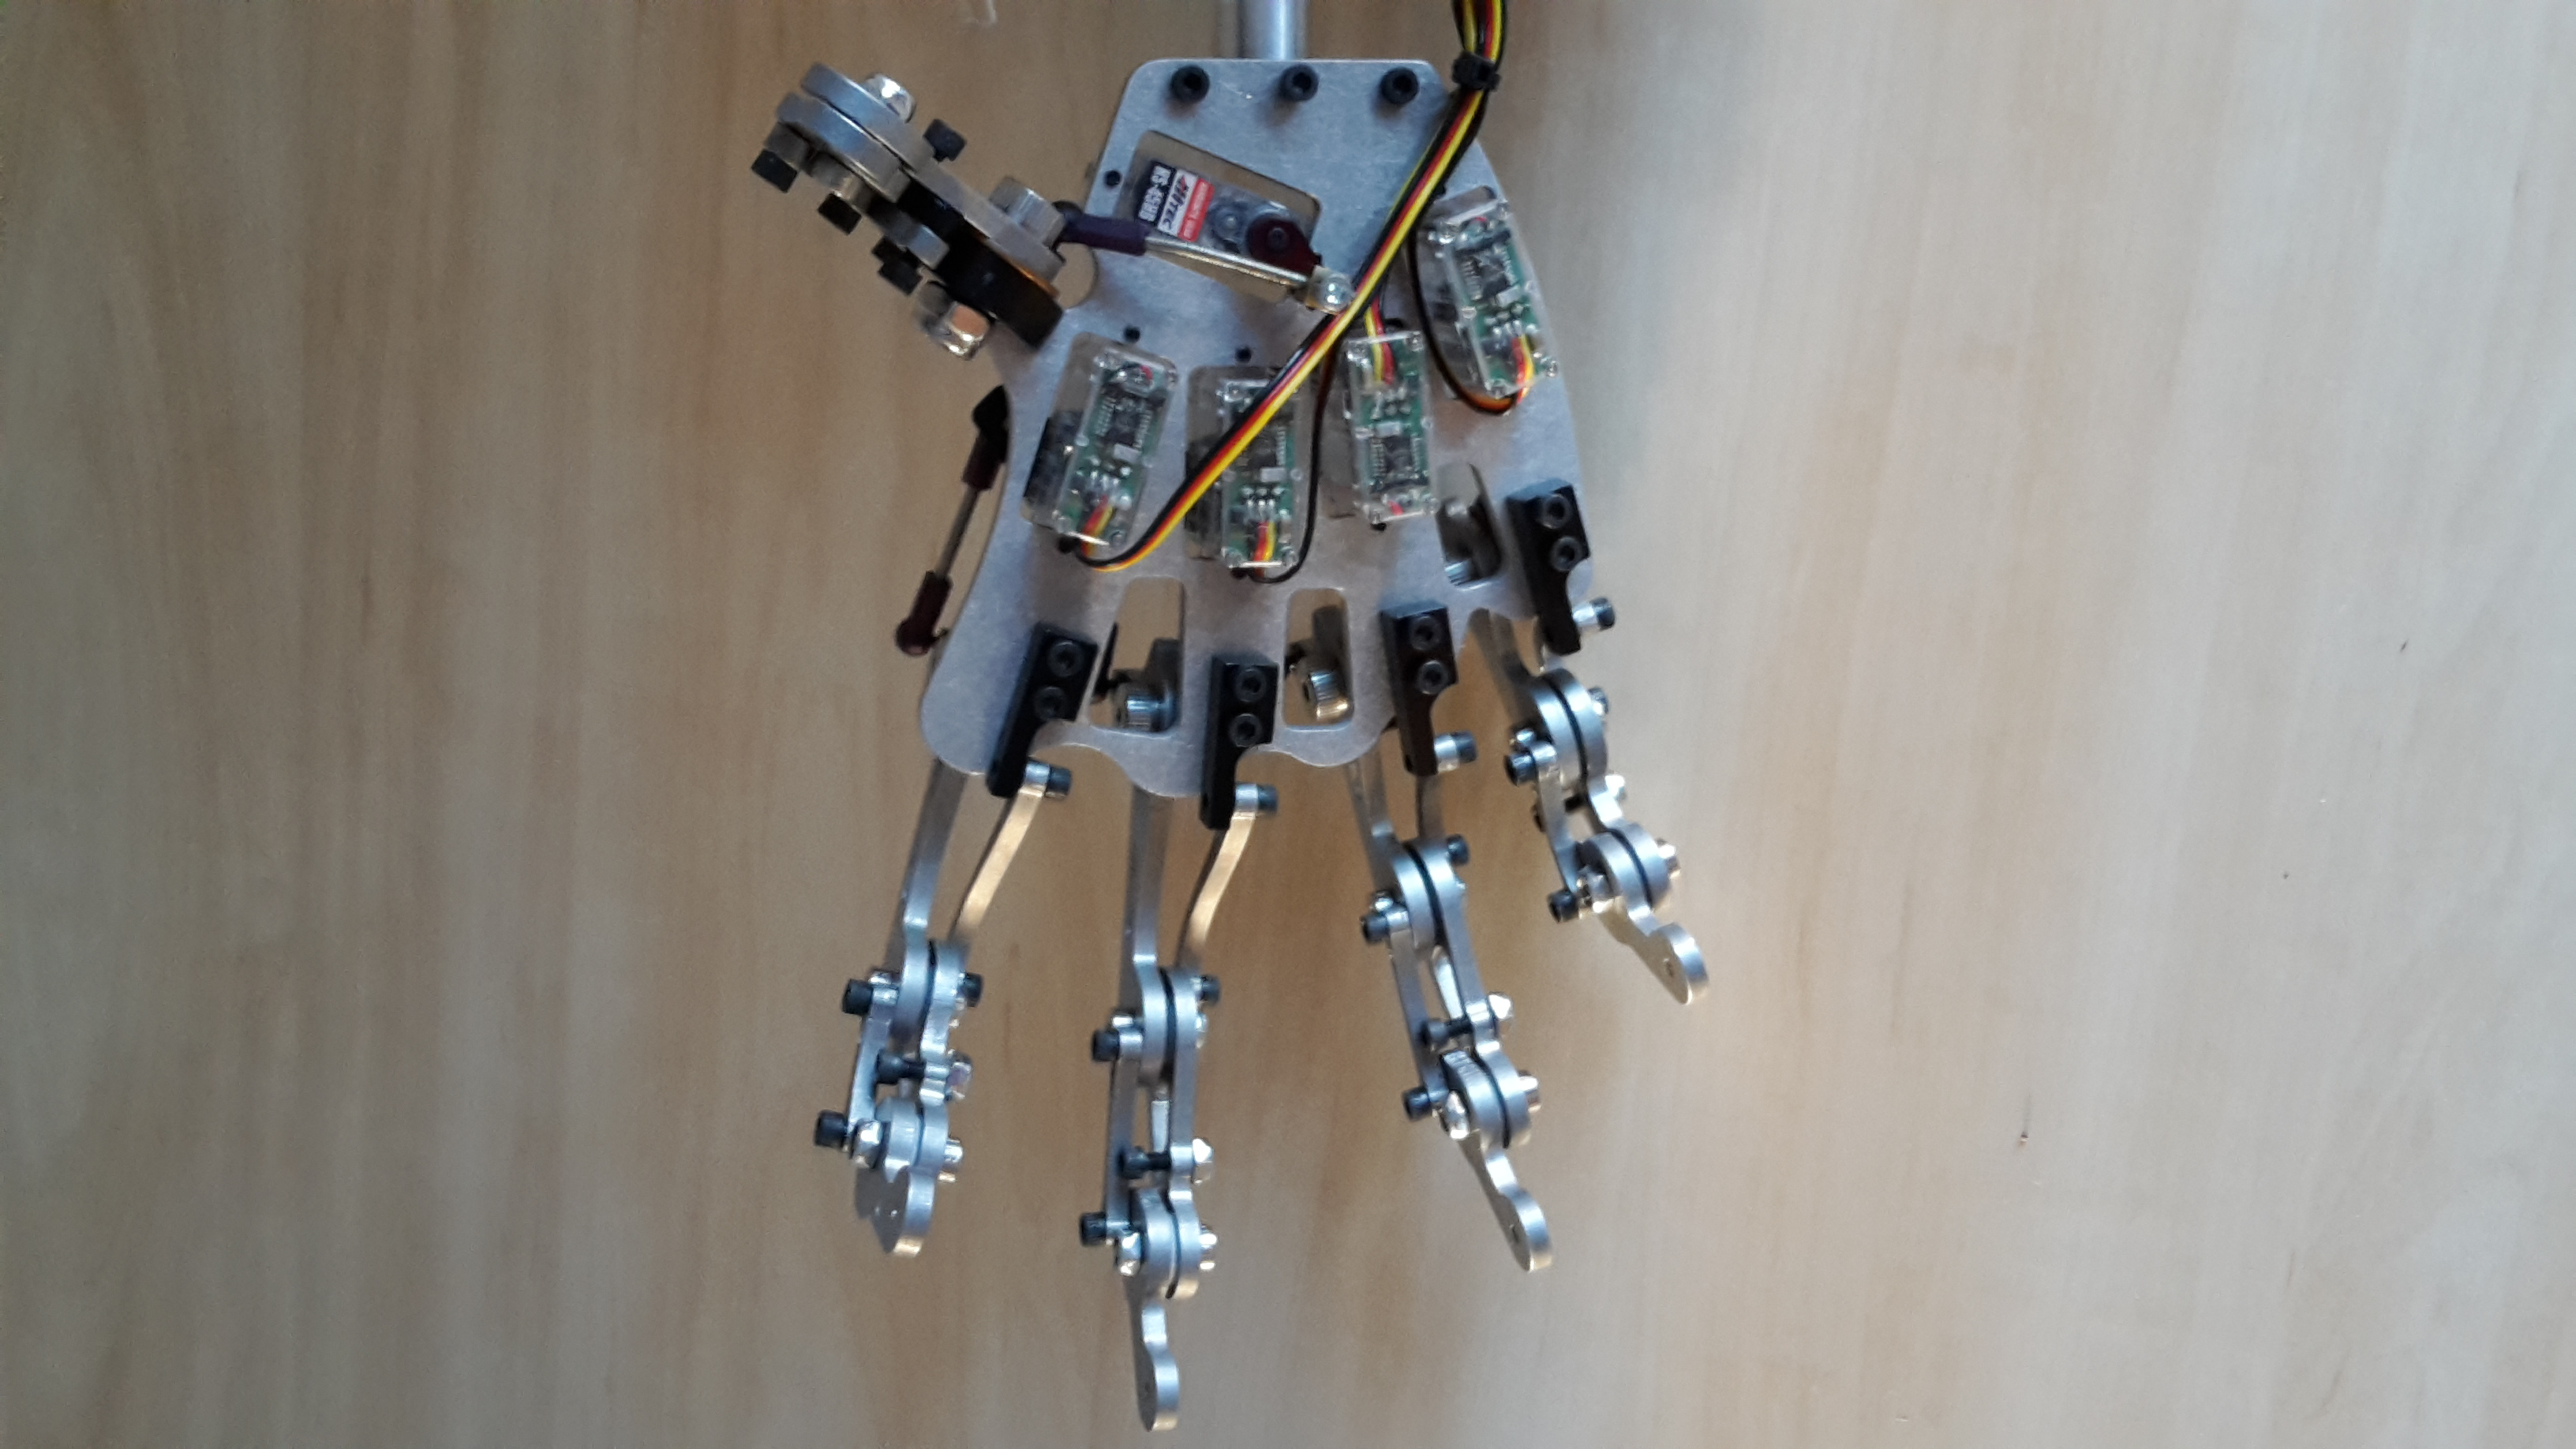
\includegraphics[trim=20cm 0cm 22cm 0cm, clip=true, totalheight=0.28\textheight, angle=-90]{photos/Day10.jpg}
	\end{tabular}
\end{figure}

\begin{figure}[H]
	\centering
	\caption{Hardware Build Progress - Arm and base built to Full build completion }
	\begin{tabular}{ll}
		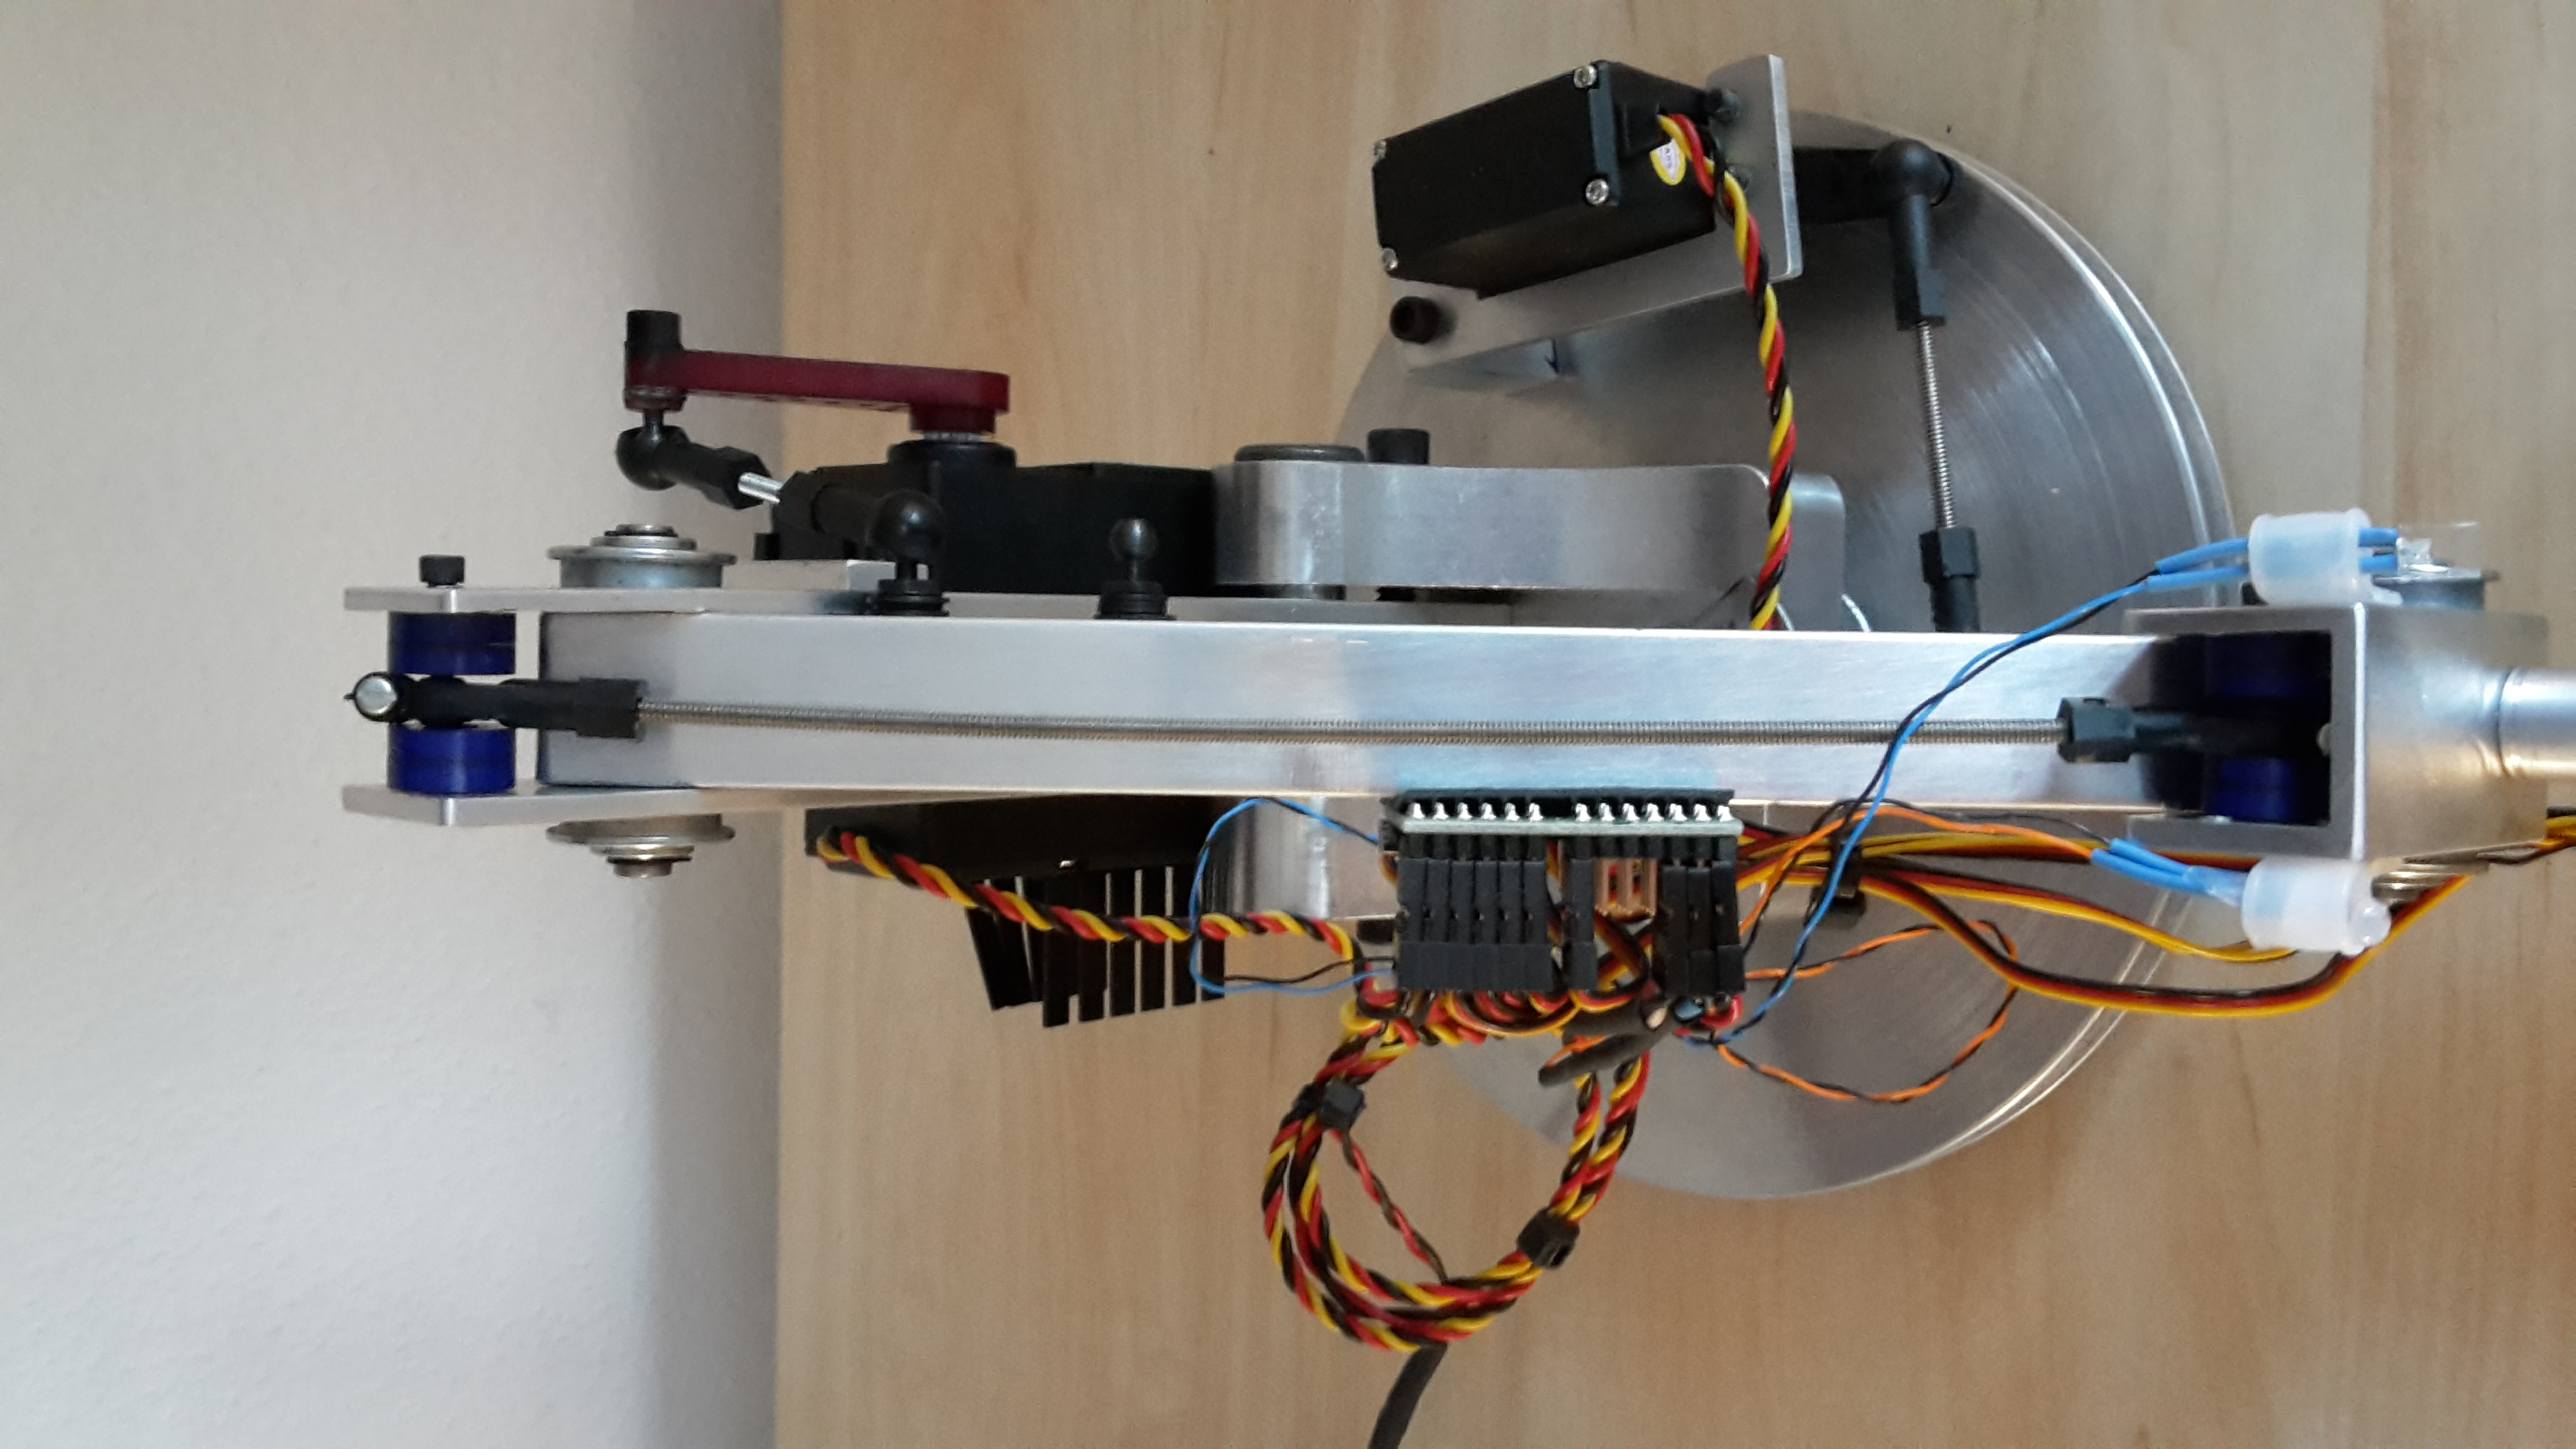
\includegraphics[trim=10cm 2cm 3cm 4cm, clip=true, totalheight=0.28\textheight, angle=-90]{photos/Day36-pt1.jpg}
		&
		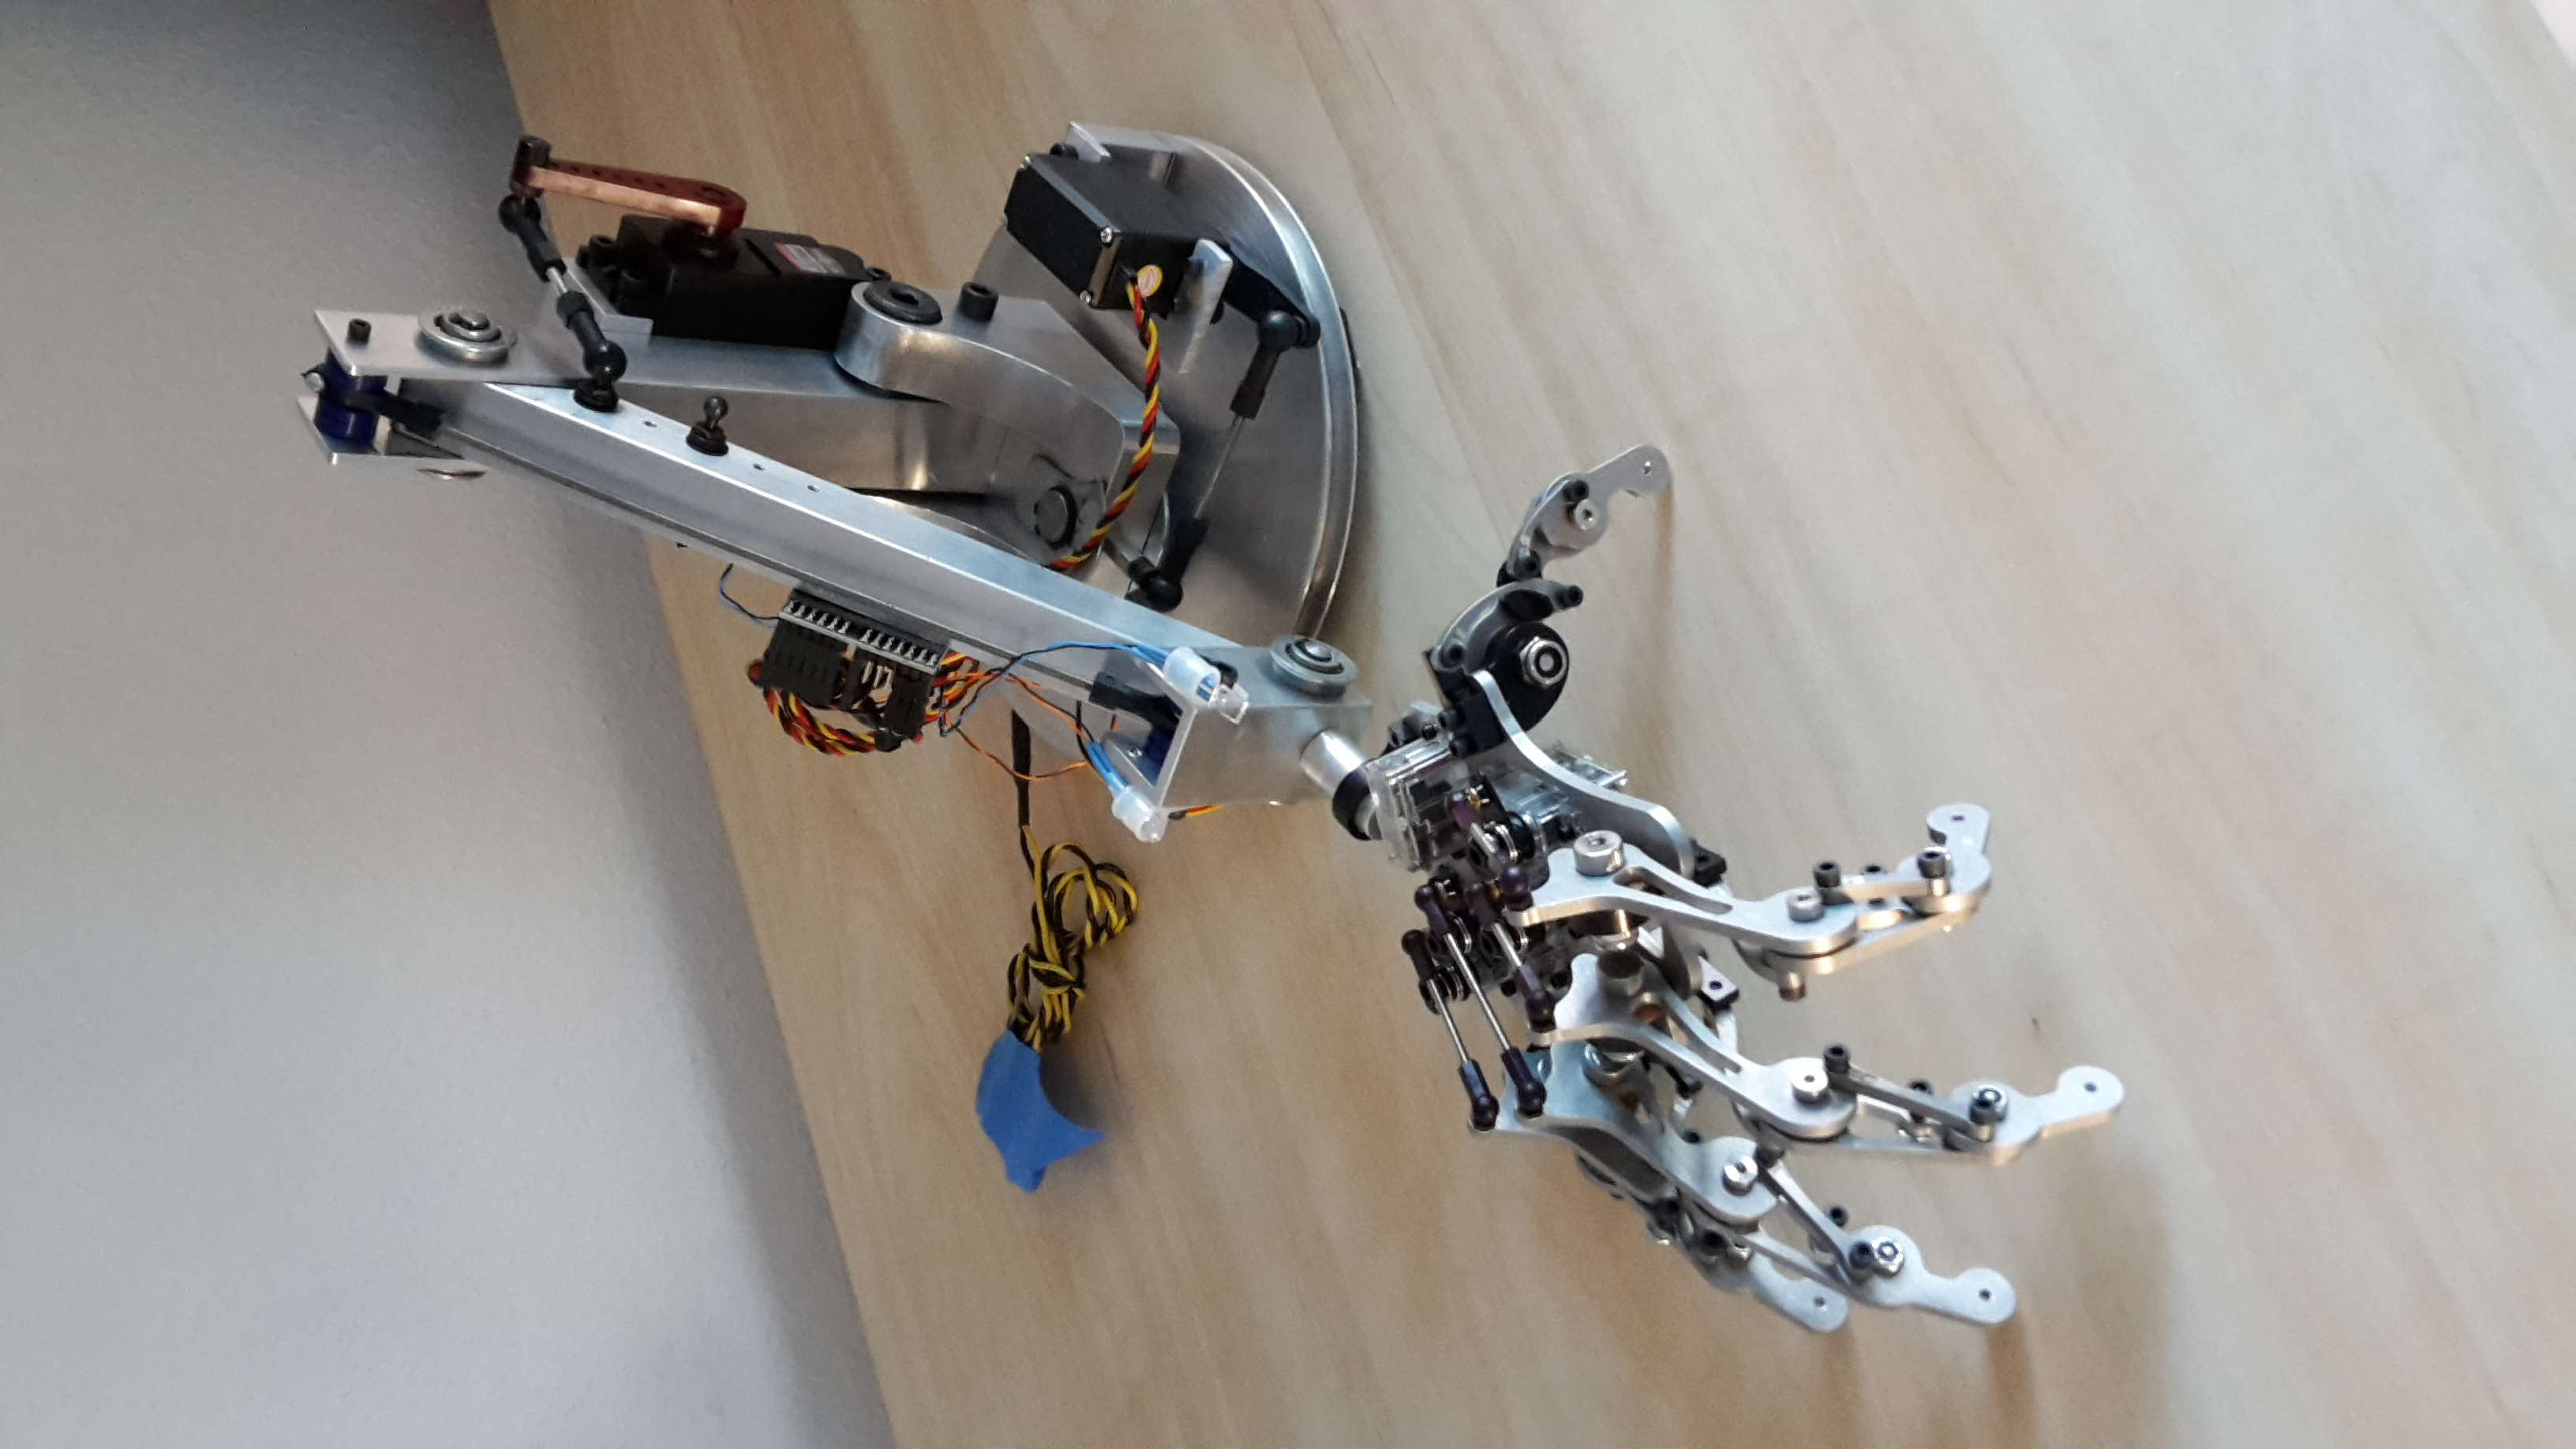
\includegraphics[trim=10cm 2cm 3cm 4cm, clip=true, totalheight=0.28\textheight, angle=-90]{photos/Day42-pt5.jpg}
	\end{tabular}
\end{figure}

The build does not go completely to plan, as the author originally estimates it will take about three full weeks, however it ends up taking just over seven. The hand and arm itself are much more complex than expected and there are several welding issues before the parts are fully positioned. 

Also, when testing the basic coding, the original servos are found to be too strong and blow the fuses and the plug, so new ones have to be ordered. 

\section{Issues and Contingencies}
The main issue, so far, is the hardware build and basic coding taking much longer, and being more complicated, than originally considered when the project was proposed. Some of the parts also take longer than expected to arrive and, as stated above, some have to be re-ordered and re-inserted into the hardware due mistakes by the author. 

The build, however, is fully completed half way through Semester 1 and the basic coding script is written and tested. The hand can currently move up, down, left, right, hold a paper coffee cup, move it and put it down. 

This means the \textbf{\textit{Must Have}} section of the \textit{MoSCoW Analysis} is fully completed and tested, leaving the more complex tracking coding  (\textbf{\textit{Should Have}} section) ready to be started. 

Unfortunately, due to a personal family bereavement, the project has to be placed on hold for a few weeks, causing an unexpected delay. Due to this delay the author has identified a few potential issues going forward into the next stage of development. They are:

\begin{itemize}		
	\item \textit{Bereavement continuing to impact productivity and efficiency}
	\item \textit{Investigation of complex coding taking longer than expected}
	\item \textit{Hardware breakdowns}
	\item \textit{Combining complex coding with the basic coding script already written}
\end{itemize}

These are considered carefully, along with the delays already occurring, so contingencies can be put in place, to ensure the project  is completed on time. 

At the end of this report are two project Gantt Charts. The first (figure 8) shows the original version included in the Project Proposal. Due to the issues and delay stated above, this plan needs to be changed. 

The Christmas holidays are originally unused so, from a contingency viewpoint, this holiday is now being included in the revised plan. The remaining tasks have also been revised, with new time-lines, to ensure the project remains on target and take into account the first two potential issues identified above. See the second Gantt chart (figure 9) for the revised plan. 

The potential hardware breakdown issue is being covered by the author ordering spare backup parts (eg sensors, servos etc) so any breakdowns can be fixed immediately, rather than having to order and wait for new parts at a later date.

And finally the potential coding issue is being dealt with by the author writing the complex code separately and testing it each time a movement, or tracking process, is written. 

This will ensure it does not interact with the basic coding, so will not cause any problems to the code already written. A decision can then be made at the end of development as to whether this should be integrated into the basic coding script, or left as a separate process.


\section{Evaluation}
Following careful reflection and evaluation the author feels that, even with the unexpected delay, good progress is being achieved with this project. 

The skill level of the author, for electronics and understanding how software code interacts with hardware, is increasing considerably and all mistakes are being learnt from and will not happen again.

The Design Document, also, turns out to be more important than originally expected. It not only ensures the hardware is built to cover all the critical movements in a human hand but, also, identifies the build as quite complex and will probably take longer than originally estimated. 

To help mitigate this issue, the build is started during the summer holidays, instead of being left until the Semester starts in September. If this was left until September the unexpected delay, mentioned above in the Issues and Contingencies section, will have fallen during the \textit{Must Have} stage of development, rather than the \textit{Should Have} stage, which will have caused a major disruption.

Instead the delay will cost the project time, but the revised Gantt chart (figure 9) shows it is still possible to accomplish the original completion date, by including Christmas and working slightly longer hours during Semester 2.

To ensure no further delays occur and any potential issues are dealt with quickly and efficiently, progress will continue to be closely monitored during the second half of the project. 

This will be achieved by the author using Trello to keep tasks on target, having regular meetings with their project supervisor and with careful project management of their available time during Semester 2.

Overall, with the revisions stated above, this project should be completed on time and provide all the requirement needed for a successful delivery.

   \begin{cmpfigure}{Original Project Gantt chart time-table\label{pplan}}
 	\centering
 	\begin{sideways}
 		\newganttchartelement{voidbar}{voidbar/.style={draw=black, top color=black!25, bottom color=black!23}}
 		
 		\begin{ganttchart}[x unit=0.45cm, vgrid, title label font=\scriptsize,canvas/.style={draw=black, dotted}]{1}{34}
 			\gantttitle{Project schedule shown for e-vision week numbers and semester week numbers}{34} \\
 			\gantttitlelist{8,...,41}{1}\\
 			\gantttitlelist{1,...,12}{1}
 			\gantttitle{Christmas}{4}
 			\gantttitlelist{1,...,9}{1}
 			\gantttitle{Easter}{4}
 			\gantttitlelist{10,...,14}{1}\\
 			
 			% Numbered in order of declaration, zero based
 			
 			\ganttbar{Project proposal}{1}{3} \\ %elem0
 			\ganttbar{Literature review}{2}{5} \\ %elem1
 			\ganttbar{Complete design and build}{2}{4} \\ %element 2
 			\ganttbar{Basic coding and testing}{4}{8}\\ %element3
 			\ganttmilestone{Basic code delivery}{9} \\ 
 			\ganttbar{Investigate Tracking}{9}{10}\\ %element 5
 			
 			\ganttbar{Tracking coding}{10}{12} %element 6 & don't include \\ to keep on same line
 			\ganttvoidbar{}{13}{16}  %don't include \\ to keep on same line
 			\ganttbar{}{17}{21}\\
 			
 			\ganttbar{Test Tracking code}{17}{22}\\
 			
 			\ganttbar{Review and Evaluation}{21}{25} \\
 			\ganttmilestone{Completed code delivery}{25} \\  
 			\ganttbar{Final report writing}{23}{30} \\  %work on writing over Easter
 			\ganttbar{Inspection preparation}{31}{34}
 			
 			\ganttlink{elem0}{elem2}
 			\ganttlink{elem1}{elem2}
 			\ganttlink{elem2}{elem3}
 			\ganttlink{elem3}{elem4}
 			\ganttlink{elem4}{elem5}
 			\ganttlink{elem5}{elem6}
 			%elem 6-7 not needed as void   
 			\ganttlink{elem8}{elem9}
 			\ganttlink{elem9}{elem10}
 			\ganttlink{elem10}{elem12}
 			\ganttlink{elem11}{elem13}
 			
 		\end{ganttchart}
 	\end{sideways}
 \end{cmpfigure}

 \begin{cmpfigure}{Revised Project Gantt chart time-table\label{pplan}}
 	\centering
 	\begin{sideways}
 		\newganttchartelement{voidbar}{voidbar/.style={draw=black, top color=black!25, bottom color=black!23}}
 		
 		\begin{ganttchart}[x unit=0.45cm, vgrid, title label font=\scriptsize,canvas/.style={draw=black, dotted}]{1}{34}
 			\gantttitle{Project schedule shown for e-vision week numbers and semester week numbers}{34} \\
 			\gantttitlelist{8,...,41}{1}\\
 			\gantttitlelist{1,...,12}{1}
 			\gantttitle{Christmas}{4}
 			\gantttitlelist{1,...,9}{1}
 			\gantttitle{Easter}{4}
 			\gantttitlelist{10,...,14}{1}\\
 			
 			% Numbered in order of declaration, zero based
 			
 			\ganttbar{Project proposal}{1}{3} \\ %elem0
 			\ganttbar{Literature review}{2}{5} \\ %elem1
 			\ganttbar{Complete design and build}{2}{4} \\ %element 2
 			\ganttbar{Basic coding and testing}{4}{8}\\ %element3
 			\ganttmilestone{Basic code delivery}{9} \\ 
 			\ganttbar{Investigate Tracking}{13}{15}\\ %element 5
 			\ganttbar{Tracking coding}{15}{23} %element 6 work over Christmas
 			\ganttbar{}{24}{24}\\  
 			\ganttbar{Test Tracking code}{20}{25}\\
 			\ganttbar{Review and Evaluation}{22}{27} \\
 			\ganttmilestone{Completed code delivery}{26} \\  
 			\ganttbar{Final report writing}{25}{30} \\  %work on writing over Easter
 			\ganttbar{Inspection preparation}{31}{34}
 			
 			\ganttlink{elem0}{elem2}
 			\ganttlink{elem1}{elem2}
 			\ganttlink{elem2}{elem3}
 			\ganttlink{elem3}{elem4}
 			\ganttlink{elem4}{elem5}
 			\ganttlink{elem5}{elem6}
 			\ganttlink{elem7}{elem8}   
 			\ganttlink{elem8}{elem9}
 			\ganttlink{elem9}{elem10}
 			\ganttlink{elem10}{elem11}
 			\ganttlink{elem10}{elem12}
 			\ganttlink{elem11}{elem13}
 			
 		\end{ganttchart}
 	\end{sideways}
 \end{cmpfigure}

  %bibliographystyle{plainyr-rev}  %shows names and dates
\pagebreak
\bibliographystyle{apalike}  %shows numbers that relate to the citations instead of names and dates
\bibliography{progress}

\end{document}
